% \documentclass[12pt, twoside]{article}
\usepackage[letterpaper, margin=1in, headsep=0.2in]{geometry}
\setlength{\headheight}{0.6in}
%\usepackage[english]{babel}
\usepackage[utf8]{inputenc}
\usepackage{microtype}
\usepackage{amsmath}
\usepackage{amssymb}
%\usepackage{amsfonts}
\usepackage[nomessages]{fp} %\FPeval{\var-name}{2*sin(pi/6)}
\usepackage{siunitx} %units in math. eg 20\milli\meter
\usepackage{yhmath} % for arcs, overparenth command
\usepackage{tikz} %graphics
\usetikzlibrary{quotes, angles, arrows, arrows.meta}
\usepackage{graphicx} %consider setting \graphicspath{{images/}}
\usepackage{parskip} %no paragraph indent
\usepackage{enumitem}
\usepackage{multicol}
\usepackage{venndiagram}

\usepackage{fancyhdr}
\pagestyle{fancy}
\fancyhf{}
\renewcommand{\headrulewidth}{0pt} % disable the underline of the header
\raggedbottom
\hfuzz=2mm %suppresses overfull box warnings

\usepackage{hyperref}

\fancyhead[LE]{\thepage}
\fancyhead[RO]{\thepage \\ Name: \hspace{4cm} \,\\}
\fancyhead[LO]{BECA / Dr. Huson / Geometry\\*  Unit 3: Parallel lines and transversals \\* 20 October 2022}

\begin{document}

\subsubsection*{3.3 Classwork: Situations with parallel lines and transversals}
\begin{enumerate}
  \item Given two parallel lines, two transversals
  \begin{multicols}{2}
    \begin{enumerate}
      \item Find $x$, $y$
      \item What relationship are you using? \\[0.5cm]
      (e.g. vertical angles, same-side exterior angles, alternate interior angles, etc.)
    \end{enumerate}
      \begin{tikzpicture}[scale=1.4]
      \draw [<->, thick] (4,2.25)--(7,2.25);
      \draw [<->, thick] (3.5,0)--(7,0);
      \draw [<->, thick] (4,-0.5)--(5.7,3);
      \draw [<->, thick] (6.5,-0.5)--(5,3);
      \node at (4.4,0.3) [right]{$73^\circ$};
      \node at (5.5,0.3) [right]{$82^\circ$};
      \node at (5.1,2.2) [below left]{$x$};
      \node at (5.5,2.2) [below right]{$y$};
    \end{tikzpicture}
  \end{multicols}

\item Find $m\angle 1$ given two parallel lines and a transversal, with
  \begin{multicols}{2}
  $\displaystyle m\angle 2 = 2x+17$ \hspace{0.75cm}$\displaystyle m\angle 7 = \frac{1}{2}(5x+5)$
  \begin{flushright}
    \begin{tikzpicture}[scale=1,rotate=-10]
      \draw [<->, thick] (3,2)--(8,2);
      \draw [<->, thick] (2,0)--(7,0);
      \draw [<->, thick] (4,-1)--(5.5,3);
      \node at (4.5,0.3) [left]{$5$};
      \node at (4.5,0.3) [right]{$6$};
      \node at (4.3,-0.3) [left]{$7$};
      \node at (4.3,-0.3) [right]{$8$};
      \node at (5.2,2) [above left]{$1$};
      \node at (5.4,2) [above right]{$2$};
      \node at (4.9,2) [below left]{$3$};
      \node at (5,2) [below right]{$4$};
    \end{tikzpicture}
  \end{flushright} 
  \end{multicols} \vspace{2cm}

\item As shown below, two lines intersect making four angles: $\angle 1$, $\angle 2$, $\angle 3$, and $\angle 4$. Given that $m\angle 1= x+32$ and $m\angle 3=2x-8$, find $m\angle 1$.
  \begin{flushright}
    \begin{tikzpicture}[scale=1, rotate=0]
      \draw [<->, thick] (1,-1)--(8,1);
      \draw [<->, thick] (3,2)--(6,-2);
      \node at (2,.3){$m\angle 1= x+32$};
      \node at (6.5,-.3){$m\angle 3=2x-8$};
      \node at (5,1){2};
      \node at (4,-1){4};
    \end{tikzpicture}
    \end{flushright}

\newpage
\item Find $m\angle 1$ given two parallel lines and a transversal, with
  \begin{multicols}{2}
  $\displaystyle m\angle 4 = 12(7x-4)$ \hspace{0.75cm}$\displaystyle m\angle 6 = 6(7x-4)$
  \begin{flushright}
  \begin{tikzpicture}[scale=1,rotate=-10]
    \draw [<->, thick] (3,2)--(8,2);
    \draw [<->, thick] (2,0)--(7,0);
    \draw [<->, thick] (4,-1)--(5.5,3);
    \node at (4.5,0.3) [left]{$5$};
    \node at (4.5,0.3) [right]{$6$};
    \node at (4.3,-0.3) [left]{$7$};
    \node at (4.3,-0.3) [right]{$8$};
    \node at (5.2,2) [above left]{$1$};
    \node at (5.4,2) [above right]{$2$};
    \node at (4.9,2) [below left]{$3$};
    \node at (5,2) [below right]{$4$};
  \end{tikzpicture}
  \end{flushright} 
  \end{multicols} \vspace{2cm}

\item An angle bisector is shown below, with $\overrightarrow{PR}$ bisecting $\angle QPS$. Given $m\angle QPR = 6x-12$ and $m\angle QPS = 10x+4$, find $m\angle QPS$.
    \begin{flushright}
    \begin{tikzpicture}[scale=0.6, rotate=30]
      \draw [<->, thick] (230:5)node[left]{$Q$} 
      --(0,0)node[above right]{$P$}
      --(110:6)node[above right]{$S$}--(110:7);
      \draw [->, thick] (0,0)--(170:7)node[below right]{$R$};
    \end{tikzpicture}
    \end{flushright}  

\item In the diagram below $\angle BOC = 7x-50$ and $\angle AOB = 4x-3$. \hfill CCSSM.8.G.B.5 \\Find $m\angle AOB$.
  \vspace{0.25cm}
  \begin{flushright}
  \begin{tikzpicture}[scale=1.3, rotate=20]
    \draw [<->, thick] (-40:3)--(0,0)--(140:3);
    \draw [<->, thick] (-3,0)--(3,0);
    \draw [->, thick] (0,0)--(0,3);
    \draw (0,0)++(0.3,0)--++(0,0.3)--+(-0.3,0);
    %\draw [fill] (-1,2.5) circle [radius=0.05] node[left ]{$B$};
    \draw [fill] (140:2) circle [radius=0.05] node[below left]{$B$};
    \draw [fill] (-2,0) circle [radius=0.05] node[below]{$A$}; 
    \draw [fill] (0,0) circle [radius=0.05] node[below left]{$O$};
    \draw [fill] (0,2) circle [radius=0.05] node[left]{$C$};
    \draw [fill] (2,0) circle [radius=0.05] node[below]{$D$};
    \draw [fill] (-40:2) circle [radius=0.05] node[below]{$E$};
  \end{tikzpicture}
  \end{flushright}


\end{enumerate}
\end{document}